\chapter{Motor Type and Control Architecture Selection}
\label{chapter:motor-control-selection}

This chapter presents the design procedure for a radiation-tolerant prototype motor driver. The discussion begins with the application context of robotic and remote-handling systems, with emphasis on electric servo actuation used in commercial, research, and CERN-related robotic platforms. This is followed by the selection of the motor type, a comparison of possible control methods, and an introduction to the vector control of brushless DC motors.

Robotic and remote-handling systems impose demanding requirements on actuators and their associated drive electronics. In contrast to simple rotary motion applications, servo systems often require accurate and repeatable motion, sufficient torque over a wide operating range, and fast dynamic response under variable loads. Therefore, the actuator is usually considered as part of a complete servo system, consisting of the motor, power electronics, feedback sensors, transmission mechanism, communication interface, and control algorithm.

The choice of motor technology depends strongly on the application requirements, including torque, speed, efficiency, cost, available power supply, control complexity, lifetime, and communication interface. In this thesis, the focus is placed on low-voltage DC-powered systems, such as battery-powered or embedded robotic platforms. For this reason, the comparison is limited to brushed DC motors, stepper motors, and brushless DC motors.

Furthermore, the radiation tolerance of the motor itself, including insulation, magnets, bearings, and mechanical materials, is not investigated in this thesis. The motor is treated as a radiation-tolerant load, while the driving electronics are considered the components under investigation.


\section{State of the Art and Application Context}
\label{sec:state-of-the-art-application-context}

Different robotic and mechatronic applications require different actuator and drive architectures. The required performance, cost, lifetime, available volume, power supply, and allowed control complexity are some of the main factors that influence the selection of the motor and the associated servo drive. As a result, robotic systems may use different motor technologies, transmission mechanisms, feedback sensors, and communication interfaces depending on the target application~\cite{TODO_general_robotic_actuation_reference}.

At CERN, robotic systems are used for inspection, remote maintenance, radiation surveys, and telemanipulation in accelerator environments where human access may be limited~\cite{TODO_CERN_robotics_reference}. Examples include [TODO: CERN robot/platform name], [TODO: CERN robot/platform name], and [TODO: CERN robot/platform name]. These systems illustrate the need for reliable remotely operated motion systems in radiation-prone areas.

Although the motor driver developed in this thesis is not designed for one specific robotic platform, such applications motivate the development of radiation-tolerant drive electronics. In these systems, the motor driver may be exposed to radiation-induced degradation or faults, while still being required to provide controlled motion, sufficient torque, and reliable communication with the control system.

Another important parameter, which is not investigated in detail in this thesis, is the communication protocol between the controller, the motor driver, and the operator interface. Several communication interfaces can be used in robotic and industrial applications, ranging from simple serial links such as RS-485, CAN, or USB, to higher-level industrial protocols such as CANopen and EtherCAT~\cite{TODO_industrial_communication_reference}. The selection of the communication interface is highly system-dependent and may require additional hardware that also needs to be qualified for operation in radiation environments.

The objective of this thesis is therefore not to design a complete robotic arm, robotic actuator, or communication system. Instead, the focus is placed on the development and evaluation of a radiation-tolerant BLDC motor driver that could serve as a building block for future robotic or mechatronic systems operating in radiation environments.


\subsection{Representative Robotic Arm Actuation Examples}
\label{sec:representative-robotic-arm-examples}

To complement the general discussion, representative robotic arm systems are considered. These examples are not intended to form an exhaustive survey of commercial robotic arms. Instead, they illustrate how different actuator technologies are used in practice depending on the target application, cost, and performance requirements.

Educational and low-cost robotic arms often use stepper motors or simple servo motors because of their simplicity and low cost~\cite{TODO_stepper_robot_arm_reference}. Research robotic arms may use smart actuators, where the motor, gearbox, encoder, driver, and communication interface are integrated into a single module~\cite{TODO_smart_servo_reference}. Industrial and collaborative robotic arms typically use closed-loop servo actuation, often based on brushless motor technology, in order to achieve higher efficiency, repeatability, and dynamic performance~\cite{TODO_industrial_robot_reference}.

These examples show that the state of the art is not defined only by the motor type. The complete actuator system includes the motor, power stage, feedback sensors, gearbox, control algorithm, and communication interface. Therefore, the development of a radiation-tolerant BLDC motor driver is relevant as a building block for future robotic and mechatronic systems operating in radiation environments.

\begin{table}[H]
    \centering
    \caption{Representative actuator approaches in robotic arm systems.}
    \label{tab:robotic-arm-actuation-examples}

    \small
    \renewcommand{\arraystretch}{1.25}

    {
    \arrayrulecolor{thesisblue}

    \begin{tabularx}{\textwidth}{
        >{\raggedright\arraybackslash}m{0.25\textwidth}
        >{\raggedright\arraybackslash}X
        >{\raggedright\arraybackslash}X
    }
        \toprule
        \textcolor{thesisblue}{\textbf{System category}} &
        \textcolor{thesisblue}{\textbf{Typical actuator approach}} &
        \textcolor{thesisblue}{\textbf{Relevance}} \\
        \midrule

        \rowcolor{thesisblue!7}
        Low-cost or educational robotic arms &
        Stepper motors or simple servo motors &
        Low cost and simple control, but limited dynamic performance and robustness under variable loads. \\

        Research robotic arms &
        Integrated smart actuators &
        Compact integration of motor, gearbox, feedback sensor, driver, and communication interface. \\

        \rowcolor{thesisblue!7}
        Industrial and collaborative robotic arms &
        Closed-loop brushless servo drives &
        High repeatability, efficiency, torque density, and dynamic response. \\

        CERN robotic and remote-handling systems &
        Radiation-aware remote actuation systems &
        Motivates the need for robust motor-drive electronics suitable for radiation-prone environments. \\

        \bottomrule
    \end{tabularx}

    \arrayrulecolor{black}
    }
\end{table}

The present thesis focuses on the last aspect: the development of radiation-tolerant motor-drive electronics suitable for BLDC motors. The work does not aim to design a complete robotic actuator or robotic arm, but rather to develop and evaluate the drive electronics that could be used as part of a larger servo system.


\subsection{Examples from Literature and Commercial Systems}
\label{sec:examples-literature-commercial-systems}

Table~\ref{tab:example-robotic-systems} lists representative systems that can be used to illustrate the range of actuator solutions found in practice. Only systems for which the actuator information is available from literature, datasheets, or manufacturer documentation should be included. When the motor technology is not explicitly stated by the manufacturer or the corresponding documentation, it should not be inferred.

\begin{table}[H]
    \centering
    \caption{Examples of robotic systems and their reported actuation approach.}
    \label{tab:example-robotic-systems}

    \small
    \renewcommand{\arraystretch}{1.25}

    {
    \arrayrulecolor{thesisblue}

    \begin{tabularx}{\textwidth}{
        >{\raggedright\arraybackslash}m{0.22\textwidth}
        >{\raggedright\arraybackslash}m{0.22\textwidth}
        >{\raggedright\arraybackslash}X
        >{\raggedright\arraybackslash}m{0.18\textwidth}
    }
        \toprule
        \textcolor{thesisblue}{\textbf{System}} &
        \textcolor{thesisblue}{\textbf{Application}} &
        \textcolor{thesisblue}{\textbf{Reported actuation approach}} &
        \textcolor{thesisblue}{\textbf{Reference}} \\
        \midrule

        \rowcolor{thesisblue!7}
        {[TODO: Example robotic arm 1]} &
        {[TODO: Educational / research / industrial]} &
        {[TODO: Stepper motor / smart servo / BLDC servo / unknown]} &
        \cite{TODO_reference_1} \\

        {[TODO: Example robotic arm 2]} &
        {[TODO: Educational / research / industrial]} &
        {[TODO: Stepper motor / smart servo / BLDC servo / unknown]} &
        \cite{TODO_reference_2} \\

        \rowcolor{thesisblue!7}
        {[TODO: Example robotic arm 3]} &
        {[TODO: Educational / research / industrial]} &
        {[TODO: Stepper motor / smart servo / BLDC servo / unknown]} &
        \cite{TODO_reference_3} \\

        {[TODO: CERN robotic system]} &
        {[TODO: Inspection / remote maintenance / teleoperation]} &
        {[TODO: Only state motor type if explicitly known]} &
        \cite{TODO_CERN_reference} \\

        \bottomrule
    \end{tabularx}

    \arrayrulecolor{black}
    }
\end{table}

The purpose of Table~\ref{tab:example-robotic-systems} is not to rank these systems, but to show that actuator selection depends on the application. Low-cost systems tend to prioritize simplicity and integration, while high-performance robotic systems require accurate closed-loop control, reliability, and dynamic response. In radiation-prone environments, an additional constraint is introduced: the drive electronics must remain functional under radiation exposure or be designed so that sensitive components are protected, replaced, or qualified.


\section{Motor Technology Selection}
\label{sec:motor-technology-selection}

Several electric motor technologies can be considered for low-voltage robotic and mechatronic systems. In this thesis, the comparison is limited to brushed DC motors, stepper motors, and brushless DC motors. These motor types are commonly used in embedded motion-control applications and can be driven from low-voltage DC supplies.

\subsection{Brushed DC Motors}
\label{sec:brushed-dc-motors}

Brushed DC motors are among the simplest electric motors to drive. Their commutation is performed mechanically using brushes and a commutator, allowing the motor speed to be controlled using a relatively simple voltage or current drive. This simplicity makes brushed DC motors attractive for low-cost applications where precise control, high efficiency, or long lifetime are not the main requirements.

However, brushed DC motors have several limitations. The mechanical brushes are subject to wear, which reduces lifetime and increases maintenance requirements. Brush contact can also introduce electrical noise and reliability concerns. For applications where the motor is difficult to access, or where long operational lifetime is required, these limitations become significant. In addition, precise position or torque control still requires external feedback sensors and a suitable control loop.

For these reasons, brushed DC motors are not selected as the target technology in this thesis.


\subsection{Stepper Motors}
\label{sec:stepper-motors}

Stepper motors provide discrete angular motion by sequentially energizing their stator windings. They are widely used in low-cost positioning systems because they can be controlled in open loop, without requiring a position sensor under normal operating conditions. Their advantages include simple control, good low-speed torque, and the ability to hold position when energized.

However, open-loop stepper motors may lose steps if the applied load exceeds the available torque. They can also exhibit vibration and reduced efficiency, especially outside their optimal speed range. In applications with variable loads, high dynamic requirements, or strict reliability constraints, open-loop control may be insufficient. Closed-loop stepper systems can improve performance, but they also increase the complexity of the system and reduce one of the main advantages of stepper motors, namely their simplicity.

Although stepper motors are suitable for many low-cost and educational robotic systems, they are not selected as the main focus of this thesis because the target application requires a motor-drive architecture more suitable for efficient closed-loop servo control.


\subsection{Brushless DC Motors}
\label{sec:bldc-motors}

Brushless DC motors replace the mechanical commutator of brushed DC motors with electronic commutation. As a result, they avoid brush wear and can provide higher efficiency, higher power density, and improved lifetime. These characteristics make BLDC motors attractive for compact servo systems, mobile robots, robotic joints, and other embedded motion-control applications~\cite{TODO_BLDC_reference}.

A BLDC motor requires a power electronic inverter and a control algorithm to energize the motor phases according to the rotor position. The rotor position can be measured using sensors, such as Hall sensors or encoders, or estimated using sensorless control methods. The increased control complexity is the main disadvantage of BLDC motors compared with brushed DC motors and stepper motors. However, this complexity also enables advanced control strategies, including closed-loop speed control, position control, torque control, and field-oriented control.

For the purposes of this thesis, BLDC motors are selected as the target motor technology because they offer a suitable compromise between efficiency, torque density, lifetime, and controllability. Compared with brushed DC motors, they avoid mechanical commutation and brush wear. Compared with open-loop stepper motors, they are more suitable for closed-loop servo control and higher dynamic performance.


\subsection{Comparison of Motor Technologies}
\label{sec:comparison-motor-technologies}

Table~\ref{tab:motor-technology-comparison} summarizes the main advantages and limitations of the motor technologies considered in this thesis.

\begingroup
\footnotesize
\renewcommand{\arraystretch}{1.25}
\arrayrulecolor{thesisblue}

% Compact vertically centered itemized cell
\newcommand{\cellitems}[1]{%
    \begin{minipage}[c]{\linewidth}
        \begin{itemize}[
            leftmargin=*,
            nosep,
            topsep=0pt,
            partopsep=0pt,
            parsep=0pt,
            itemsep=0pt
        ]
            #1
        \end{itemize}
    \end{minipage}
}

\begin{longtable}{
    @{}
    >{\centering\arraybackslash}m{0.15\textwidth}
    >{\raggedright\arraybackslash}m{0.245\textwidth}
    >{\raggedright\arraybackslash}m{0.245\textwidth}
    >{\raggedright\arraybackslash}m{0.245\textwidth}
    @{}
}

\caption{Comparison between brushed DC, brushless DC and stepper motors.}
\label{tab:motor-technology-comparison} \\

\toprule
&
\multicolumn{1}{c}{\textcolor{thesisblue}{\textbf{Brushed DC}}} &
\multicolumn{1}{c}{\textcolor{thesisblue}{\textbf{Brushless DC}}} &
\multicolumn{1}{c}{\textcolor{thesisblue}{\textbf{Stepper}}} \\
\midrule
\endfirsthead

\caption[]{Comparison between brushed DC, brushless DC and stepper motors. \textit{(continued)}} \\

\toprule
&
\multicolumn{1}{c}{\textcolor{thesisblue}{\textbf{Brushed DC}}} &
\multicolumn{1}{c}{\textcolor{thesisblue}{\textbf{Brushless DC}}} &
\multicolumn{1}{c}{\textcolor{thesisblue}{\textbf{Stepper}}} \\
\midrule
\endhead

\midrule
\multicolumn{4}{r}{\textit{Continued on next page}} \\
\endfoot

\bottomrule
\endlastfoot

\rowcolor{thesisblue!7}
\textcolor{thesisblue}{\textbf{Speed range}} &
\cellitems{
    \item Maximum speed limited by mechanical friction and wear of brushes
}
&
\cellitems{
    \item Typically, for the same voltage, the maximum speed is much higher
}
&
\cellitems{
    \item Maximum speed is very limited
    \item Torque--speed curve rapidly decreasing
}
\\

\textcolor{thesisblue}{\textbf{Control method}} &
\cellitems{
    \item No control required for basic driving, only PWM
    \item Feedback and additional sensors/circuits are required for precise speed/position control
}
&
\cellitems{
    \item Closed-loop control required
    \item Components and circuits for speed/position control are mandatory
    \item Control algorithms need to be implemented
}
&
\cellitems{
    \item Open-loop control for traditional driving in discrete steps
    \item Closed-loop control with encoders can be implemented for more advanced control
}
\\

\rowcolor{thesisblue!7}
\textcolor{thesisblue}{\textbf{Heat dissipation}} &
\cellitems{
    \item Poor, heat is concentrated in the internal mechanical part of the motor
    \item Friction produces more heat
}
&
\cellitems{
    \item Good, heat is generated in the external stator, making it very easy to cool
}
&
\cellitems{
    \item Good, as long as the motor is operated at nominal current
}
\\

\textcolor{thesisblue}{\textbf{Durability and reliability}} &
\cellitems{
    \item Shorter lifetime
    \item Periodic maintenance and cleaning due to brush and commutator wear and remnants
}
&
\cellitems{
    \item Long lifetime
    \item Low maintenance required
}
&
\cellitems{
    \item Long lifetime
    \item High reliability, no brushes and no Hall sensors
}
\\

\rowcolor{thesisblue!7}
\textcolor{thesisblue}{\textbf{Electronics BOM}} &
\cellitems{
    \item Low
    \item Increasing if a control loop is employed
}
&
\cellitems{
    \item High
}
&
\cellitems{
    \item Low
    \item Increasing if encoders are employed
}
\\

\textcolor{thesisblue}{\textbf{Ideal when}} &
\cellitems{
    \item Low cost, driving simplicity and easy integration are desired
}
&
\cellitems{
    \item Efficiency, controllability and longevity are a priority
}
&
\cellitems{
    \item Precision, high torque at lower speeds and high holding torque are a priority
}
\\

\end{longtable}

\arrayrulecolor{black}
\endgroup

From this comparison, BLDC motors are selected for the proposed radiation-tolerant motor driver. Although their control is more complex than that of brushed DC or stepper motors, this complexity is justified by their efficiency, lifetime, and suitability for closed-loop operation. These properties are especially relevant for robotic and remote-handling systems, where the actuator may be difficult to access and reliable operation is required.


\section{Justification for a Radiation-Tolerant BLDC Motor Driver}
\label{sec:justification-radtol-bldc-driver}

The development of a radiation-tolerant BLDC motor driver is motivated by the need for reliable actuation in environments where conventional electronics may suffer from radiation-induced degradation or faults. Objectively, stepper motors have the advantage that they can perform relatively precise position control and produce high torque in open-loop operation. At first, this appears attractive because reducing the final bill of materials also reduces the number of possible failure points. However, as will be shown later, the motor driver system can suffer from radiation-induced degradation due to both total ionizing dose and displacement damage. As a result, the characteristics of the semiconductors can change, modifying the behavior of the system. In addition, the microcontroller may suffer from single-event effects, which can compromise controllability without the operator being immediately aware of the fault.

For these reasons, the appropriate control approach for this application is a closed-loop system. The advantages can be summarized as follows:

\begin{enumerate}
    \item The controller can compensate for the long-term degradation of the system.
    \item Several diagnostic and fault-coping mechanisms can be implemented.
    \item The degradation of the system can be made observable by the operator.
\end{enumerate}

For a closed-loop control implementation, additional feedback components are necessary regardless of the selected motor type. These include current-monitoring circuits, position or speed sensors, and the associated signal-conditioning and processing electronics.

Therefore, the selected type of motor for this development is the BLDC motor. A servo application with a BLDC motor will be very efficient and provide a lot of benefits in terms of control performance. The BLDC motor is also a motor that is suitable for every kind of application as changing a bit the control software, it can be very efficient in torque, velocity, and position control. Furthermore, as it is a three-phase motor, its control system, hardware and software, can be implemented so that it can support driving AC Permanent-Magnet Synchronous Motors (PMSM), AC Induction Machines (ACIM), and even stepper motors.

Qualifying a BLDC closed-loop control system, even though it is perhaps the most challenging approach, it is expected to reveal the most vulnerabilities. Moreover, developing a system for a BDC motor is also something that would make a lot of sense, especially since it is used in robotic operations, but qualifying a BDC motor system would mean that more components and software complexity will have to be added and tested in the future.

The thesis will focus on the development of a BLDC motor driver system at a hardware and software level.

\section{Control Methods for BLDC Motors}
\label{sec:bldc-control-methods}

BLDC motors can be controlled using different methods, depending on the required performance, available sensors, computational resources, and implementation complexity. The most common approaches include trapezoidal control, sinusoidal control, and field-oriented control.

\subsection{Trapezoidal Control}
\label{sec:trapezoidal-control}

Trapezoidal control, also known as six-step commutation, is one of the simplest methods for driving BLDC motors. In this method, two motor phases are energized at a time, while the third phase is left Hi-Z. The commutation sequence is determined from the rotor position, which can be measured using Hall sensors or estimated from the Back-EMF.

\begin{figure}[H]
  \centering
  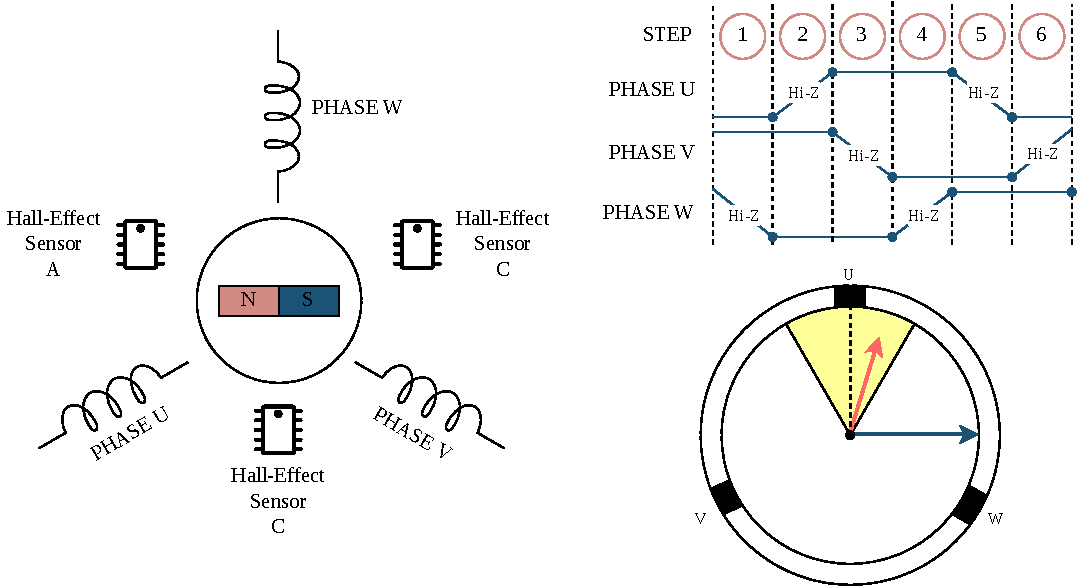
\includegraphics[width=\textwidth,keepaspectratio]{03_MotorControlSpecifications/images/Trapezoidal_Control.pdf}
  \caption{Trapezoidal control}
  \label{fig:trap-control}
\end{figure}

The main advantage of trapezoidal control is its simplicity. It requires relatively low computational resources and is suitable for applications where moderate torque ripple and acoustic noise are acceptable. And it can prove very effective at high speeds. However, because the phase currents are not sinusoidal, trapezoidal control can produce torque ripple, vibration, and reduced performance at low speed. That makes it suitable for applications like fans, or whatever.

\subsection{Sinusoidal Control}
\label{sec:sinusoidal-control}

Sinusoidal control improves upon trapezoidal control by applying sinusoidal phase currents to the motor windings. This reduces torque ripple and can improve smoothness of operation. However, sinusoidal control requires more accurate rotor position information and more complex current regulation compared with six-step commutation.

The idea is to modulate PWM signal in order to control the effective voltage on the motor phases. Since motor phases are inductive elements the current resists the change and thus it acts as an RL filter that smooths out the wave signal and the current is sinusoidal.

\begin{figure}[H]
  \centering
  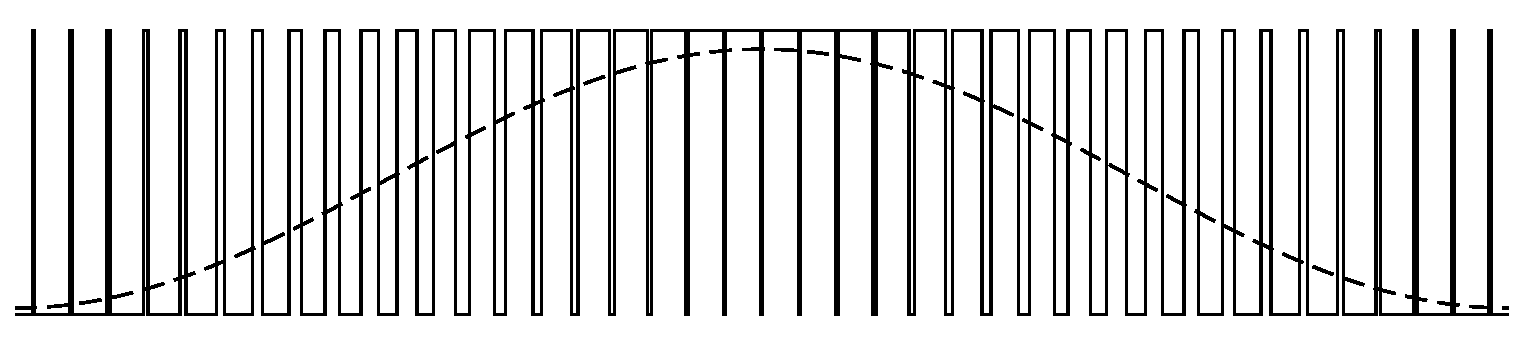
\includegraphics[width=\textwidth,keepaspectratio]{03_MotorControlSpecifications/images/Sinusoidal_PWM_Diagram.pdf}
  \caption{Sinusoidal PWM and the current that the motor sees in its windings}
  \label{fig:sinusoidal-pwm}
\end{figure}

Although sinusoidal control can provide smoother operation, it does not fully decouple the torque-producing and flux-producing components of the stator current. For applications requiring high-performance torque control, field-oriented control is generally preferred.

\subsection{Field-Oriented Control}
\label{sec:field-oriented-control}

Field-oriented control, also known as vector control, transforms the three-phase stator currents into a rotating reference frame aligned with the rotor magnetic field. This allows the motor currents to be separated into two components: one associated with the magnetic flux and one associated with torque production. As a result, the BLDC motor can be controlled in a manner similar to a separately excited DC motor.

The main advantage of field-oriented control is its ability to provide smooth and efficient torque control over a wide operating range. This makes it suitable for servo applications where accurate current, velocity, or position control is required. The disadvantage is the increased computational complexity and the need for accurate current measurement, rotor position information, and coordinate transformations.

For this thesis, field-oriented control is considered the most relevant control method because it enables high-performance closed-loop operation of BLDC motors. The following sections introduce the mathematical transformations and control structure used for vector control.

\subsubsection{Space-Vector Modulation PWM}

The Space-Vector PWM (SVPWM) waveform generation is one of the core elements of FOC. 

\subsubsection{Clarke \& Park Transformations}

The Clarke and Park transformations as well as their inverse are another very important aspect of the FOC. As the core idea of the FOC is that we move from the three-dimensional stationary abc-frame to the rotational dq-frame. In order to provide some context on the transformations, the mathematical definition accompanied by the application to motor phases will be shown.

\textbf{Clarke Transformation} \\
In a 3-phase sinusoidal system, the currents and voltages are typically $120^\circ$ apart. This means that there is redundant "information" in the voltage $\textbf{V} = \left[V_a, V_b, V_c\right]$ and current $\textbf{I} = \left[I_a, I_b, I_c\right]$ vectors. 

The idea behind this mathematical operation (that was modeled by Edith Clarke) is to simplify the three-dimensional reference frame that is used in three-phase inverters (the so called abc-frame) and project it into an equivalent two-dimensional stationary frame, usually mentioned as $\alpha\beta$-frame. That means to reduce the system complexity by removing the redundant information.

Finally, the most important takeaway is to intuitively understand that both the $120^\circ$ abc-frame and the derived $\alpha\beta$-frame are stationary, and that means that the frame remains fixed to the stator. So, informally, we can say that the calculations happen from the "stators'" point of view. The Clarke transformation is used together with the Park transformation to transform a 3-phase motor model into a dq-frame.

\textbf{Park Transformation} \\
These transformations unlock one of the main advantages of field-oriented control (FOC): the ability to decouple magnetic flux control from torque control. In FOC, the reference frame is chosen such that the flux-producing and torque-producing components can be controlled independently. Since the torque generated by two interacting magnetic field vectors is proportional to the magnitude of their cross product, maximum torque is obtained when the rotor and stator magnetic field vectors are orthogonal:

\begin{equation*}
    \boldsymbol{\vec{T}} \propto 
    \boldsymbol{\vec{B}}_{\text{rotor}} \times 
    \boldsymbol{\vec{B}}_{\text{stator}}
\end{equation*}

with maximum torque when

\begin{equation*}
    \theta = 90^\circ
\end{equation*}

The decoupling is accomplished by the Park transformation that transforms the stationary $\alpha\beta$-frame into a rotating dq-frame, where d stands for direct and q for quadratic. For BLDC/PMSM this frame is typically fixed to the rotor meaning that intuitively the calculations happen from the rotor's point of view. This can be visualized by thinking that we don't modulate the stator anymore but directly the rotor and its axis d and q.

Of course, more context about the system is needed since it is necessary to know the angle of the rotors' permanent magnets at each step of the algorithm, once per PWM period for FOC. For that, and given that the pole-pairs of the motor are $pp\geq1$, the electrical angle is utilized which is defined as the mechanical angle multiplied by the number of pole pairs

\begin{equation*}
    \theta_e = \theta_m \cdot N_{pole-pairs} [deg]
\end{equation*}

\subsubsection{The PID Controller}

The PID controller is another core component of FOC. Even though more performant and modern alternatives exist, PID is the classic controller that is used internally by the FOC control loops. Since it is well known to most engineers it will only be briefly presented.

\subsubsection{Startup System Calibration}

\section{Selected Approach}
\label{sec:selected-approach}

Among the aforementioned control algorithms, the selected approach is Field-Oriented Control. For servo applications, and more specifically for robotic arm applications, FOC is a very suitable choice, as it generally provides the best behaviour under dynamic loading conditions. It also has a wider range of applications, since it can be used for torque, velocity, and position control modes. Last but not least, as an algorithm, it can be applied to many different types of motors, such as DC and AC PMSMs, AC Induction Machines (ACIMs), and even stepper motors.

As already mentioned, selecting a closed-loop algorithm is necessary when dealing with harsh environments with high radiation levels. The electronics will naturally degrade due to TID and DD, and a feedback loop may be adequate to compensate for some of these errors, for example current leakage. Furthermore, failures attributed to SEE would not be possible to detect if the system was operating in open-loop.

FOC, or spin-offs of FOC, are currently the industry standard in PMSM motor control due to their versatility and the additional control options they enable.

Even if FOC is not considered in the future, qualifying a system of this level of complexity under radiation would still provide confidence in the feasibility of simpler systems, where part of the control complexity is removed.